\section{Problem Formulation}
\label{sec:formulation}

\paragraph{Skills, executions and token positions.}
We supply instructions directly, holding skill selection fixed.
For the same question, the \emph{donor} uses the correct skill and the
\emph{receiver} uses length-matched text from a fixed unrelated skill
(Appendix~\ref{app:detail}). Skill positions form the \emph{source span}
$\mathcal I$, including instructions such as a calculator's formula but
excluding the question. \emph{Readers} $\mathcal J$ are subsequent prompt
and generated-token positions. Receiver denotes an execution, while
reader denotes a token position. Causal attention blocks access to future
tokens, so earlier positions cannot read the skill.

Layers are indexed from zero. The model processes prompt tokens during
\emph{prefill} and generates answer tokens during \emph{decoding}.
We use greedy decoding, which selects the highest-probability next token.
We compare what source-state transfer restores in the receiver with what
blocking source attention removes from the donor.

% Queue the design graphic within the methods, ahead of the next page top.
\begin{figure*}[t]
\centering
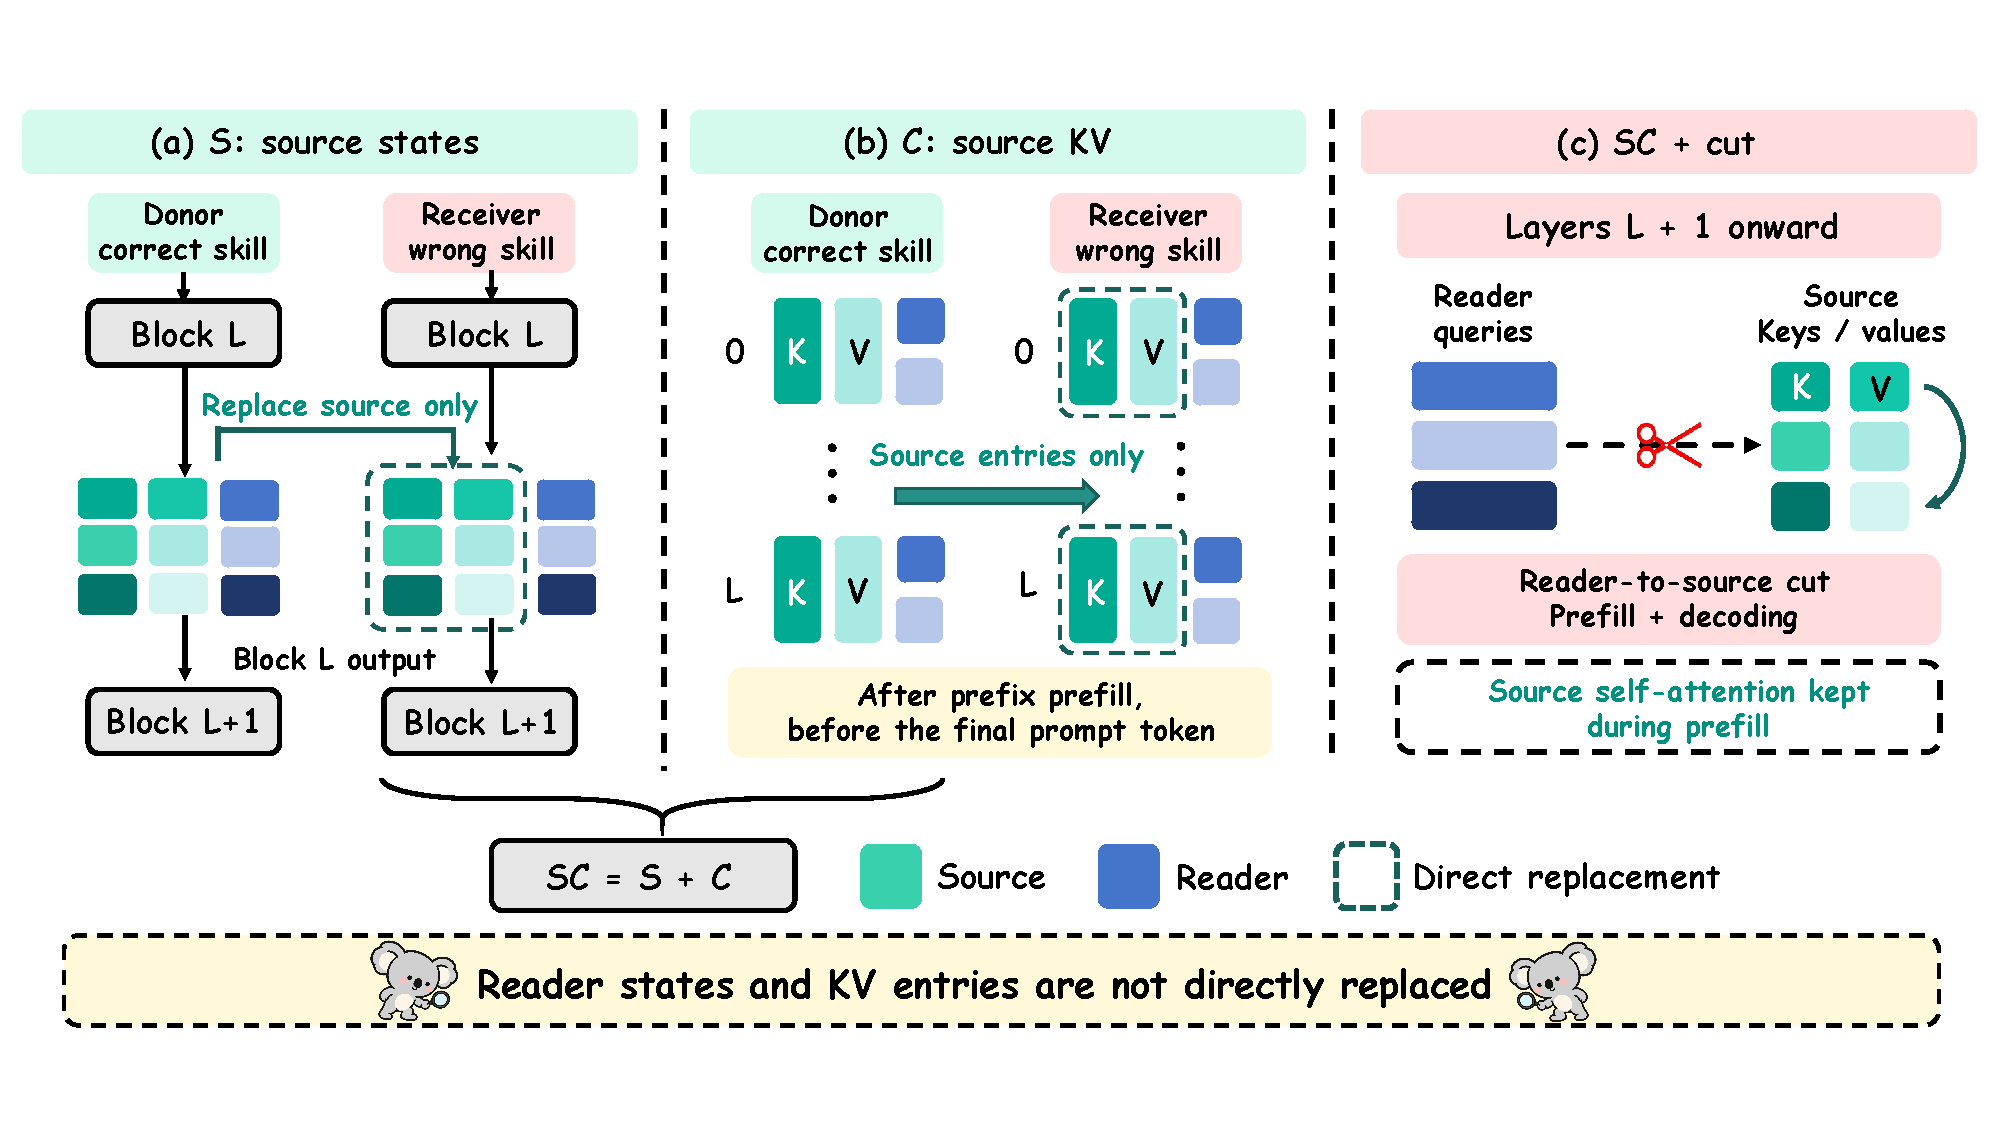
\includegraphics[width=\textwidth]{fig-intervention-design.pdf}
\caption{Receiver interventions and their timing.
(a) $S$ replaces source states at block $L$ during prefix prefill.
(b) $C$ copies source KV at layers $0$ through $L$ after prefix prefill.
$SC$ combines both writes before recomputing the final prompt token and generating.
(c) $SC+\mathrm{cut}$ installs its mask before prefill and blocks skill
reading from $L+1$ during prefill and decoding, retaining within-skill attention.
Reader states and KV are not directly replaced. Figure~\ref{fig:mechanism}(b)
instead cuts attention in the original correct-skill run.}
\Description{Three panels illustrate source-state replacement at block L's
output, source-key/value replacement at layers zero through L, and joint
replacement with a reader-to-source attention cut from layer L plus one.
Green cells mark source positions, blue cells mark readers, and dashed teal
outlines mark direct replacements. The cut applies during prefill and
decoding while source self-attention remains unmasked during prefill.}
\label{fig:design}
\end{figure*}

\paragraph{Hidden-state transfer.}
Each Transformer block updates the token vectors. Let $H^L$ be its output
at layer $L$, also called residual states, with subscripts $D/R$ for
donor/receiver. State replacement $S$ writes
\begin{equation}
S:\qquad H_R^L[\mathcal I]\leftarrow H_D^L[\mathcal I].
\label{eq:inject}
\end{equation}
During prefill, the receiver continues from this write, retaining other
positions' states at layer $L$.

\begin{samepage}
\paragraph{Blocking attention to the skill.}
\emph{Cumulative source-attention knockout} blocks access to source
positions from layer $L$ onward in the original correct-skill run.
Attention uses query vectors to score keys and combines value vectors
with the resulting weights. For the query-to-key score $z^\ell_{ij}$,
including the causal mask, each layer $\ell\ge L$ uses
\begin{equation}
\widetilde z^\ell_{ij}=
\begin{cases}
-\infty,&j\in\mathcal I,\\
z^\ell_{ij},&j\notin\mathcal I.
\end{cases}
\label{eq:knockout}
\end{equation}
\end{samepage}
Softmax converts these scores into weights, assigning zero to blocked
positions and normalizing the rest. The cut applies to all query positions
and all heads, the block's parallel attention components, during prefill
and decoding. It blocks both skill reading and attention within the skill,
measuring aggregate source-attention dependence.

Figure~\ref{fig:design} also introduces source-cache replacement ($C$)
and joint repair ($SC$), defined below.



\paragraph{Recovery and dependence.}
Write $a_D$, $a_R$ and $a_I$ for answer accuracy under the donor, receiver
and an intervention $I$. Recovery is the fraction of the donor's gain
restored in the receiver:
\begin{equation}
\rho(I)=\frac{a_I-a_R}{a_D-a_R}.
\label{eq:rho}
\end{equation}
For $a_D>a_R$, $\rho=1$ restores the gain and $\rho>1$ exceeds donor
accuracy. We write $\rho(L)$ for state replacement at layer $L$.
All accuracies use the same items and the transfer protocol's own
baselines (Section~\ref{sec:setup}).

For knockout, let $q(L)$ be the fraction of eligible, originally correct
answers that remain correct. Source-attention dependence is
\begin{equation}
d(L)=1-q(L).
\label{eq:dependence}
\end{equation}
Higher $d$ means more correct answers lost. We compare receiver recovery
$\rho$ and donor dependence $d$ on common eligible IDs, retaining each
test's baselines. A paired-outcome check asks whether transfer and knockout
both yield incorrect answers on the same questions.

\paragraph{Depth boundaries.}
After establishing effective early transfer, we summarize the curves by
their first half-effect boundaries:
\begin{equation}
\begin{aligned}
T&=\min\{L:\rho(L)<0.5\},\\
R&=\min\{L:d(L)\le0.5\},\qquad \Delta=R-T.
\end{aligned}
\label{eq:boundaries}
\end{equation}
When both crossings exist, $\Delta$ measures their separation.
The weak-transfer, strong-dependence set
$\mathcal W=\{L:\rho(L)<0.5,\ d(L)>0.5\}$ can contain several intervals.
Figure~\ref{fig:transferreading} retains later threshold crossings.

\paragraph{The execution state before generation.}
For one question, split the complete $n$-token prompt before its last token
$u_*$. The processed prefix has positions $\mathcal P=\{0,\ldots,n-2\}$,
including the skill and question. Let
$\overline{\mathcal I}=\mathcal P\setminus\mathcal I$.
Attention reuses cached keys and values for these processed tokens
\citep{shazeer2019fast}. At this point, define
$\mathcal C_X^\ell[\mathcal I]=(K_X^\ell[\mathcal I],V_X^\ell[\mathcal I])$,
collect all layers as $\mathcal C_X[\mathcal I]$, and write
$\mathcal B_X=\mathcal C_X[\overline{\mathcal I}]$ for the other prefix
caches. With model parameters $\theta$, positions, stopping rule and
greedy decoding fixed, the continuation is
\begin{equation}
\hat y_X=\mathcal G_{\theta,M_X}
       (u_*,\mathcal C_X[\mathcal I],\mathcal B_X).
\label{eq:continuation}
\end{equation}
Here $M_X$ specifies attention masks, and $\mathcal G$ includes computing
$u_*$ and generating the answer from both source and other prefix caches.

\paragraph{Cache replacement and joint repair.}
After prefix prefill and before computing $u_*$, cache replacement writes
\begin{equation}
C:\quad \mathcal C_X^\ell[\mathcal I]
 \leftarrow\mathcal C_D^\ell[\mathcal I],\qquad 0\le\ell\le L.
\label{eq:cache}
\end{equation}
The prefix uses no state write for $C$ ($X=R$), or a block-$L$ write for
$SC$ ($X=S$). Cache replacement preserves other prefix entries, giving
$\mathcal B_C=\mathcal B_R$ and $\mathcal B_{SC}=\mathcal B_S$.
Indirect effects of $S$ can change $\mathcal B_S$ relative to $\mathcal B_R$.
Under the causal assumptions in Appendix~\ref{app:cache-coverage}, ideal
state replacement reconstructs source KV at layers above $L$. The explicit
cache write supplies layers $0$ through $L$, giving donor-aligned source
caches under $SC$ while retaining the receiver's other prefix caches
$\mathcal B_S$. Figure~\ref{fig:design} shows the write schedule.

Exact copying removes the replaced entries' contribution to squared
cache distance from the donor. Appendix~\ref{app:behavior-recovery} derives this identity
and a sufficient condition for matching donor outputs under bounded
changes in token scores.

\begin{samepage}
\paragraph{Reading cuts and their timing.}
A \emph{skill-reading cut} blocks reader-to-source attention.
A \emph{within-skill attention cut} blocks source-to-source attention.
In $SC+\mathrm{cut}$, the reading mask is
\begin{equation}
\widetilde z^\ell_{ij}=
\begin{cases}
-\infty,&\ell\ge L+1,\ i\in\mathcal J,\ j\in\mathcal I,\\
z^\ell_{ij},&\text{otherwise}.
\end{cases}
\label{eq:reading-cut}
\end{equation}
\end{samepage}
It is installed before prefix prefill and persists during decoding.
Source-to-source attention remains unmasked, but reader computation can
change already during prefill. Consequently both $M_X$ and
$\mathcal B_X$ in Eq.~\eqref{eq:continuation} can differ from $SC$.
The separate original-run path tests start their cuts at $L$, not $L+1$.
Adding a within-skill cut to a persistent reading cut is structurally
redundant for the output (Appendix~\ref{app:mechanism}).

\paragraph{Repair contrasts.}
On a fixed evaluation set, we measure the cache gain $SC-S$ and the
reading-cut loss $SC-(SC+\mathrm{cut})$ in accuracy points.
The interaction $\Gamma$ compares the joint gain with the sum of the
individual gains. Appendix~\ref{app:mechanism} gives their formulas.
